
	
		% Schreiben einer Labview VI, die Amplitudenmodulation mit Hilfe der Sinus VI durchführt
		% falsche Verkabelung für Ausgabe des Signals über Soundkarte (Fehler zunächst nicht erkannt)
			% -> Verwendung des Funktionsgenerators für Modulation
		% Messstruktur um Demodulation für AM erweitern
		
		Zu Beginn des dritten Tages wurde die Arbeit an der Messstruktur fortgesetzt.
		Abb. \ref{fig:messstruktur} stellt das Endprodukt für diesen Aufgabenteil dar.
		\newpage
		\thispagestyle{empty}
		\begin{figure}[H]
			\centering
			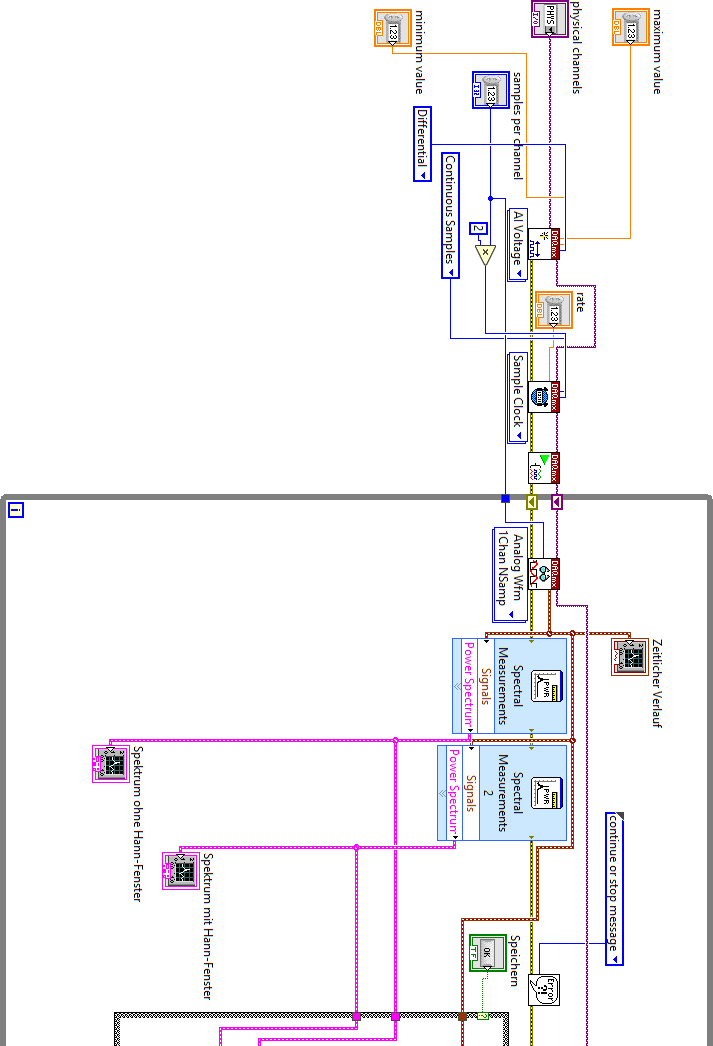
\includegraphics[width=\textwidth]{pic/messstruktur1.png}	
		\end{figure}
		
		\begin{figure}[H]
			\centering
			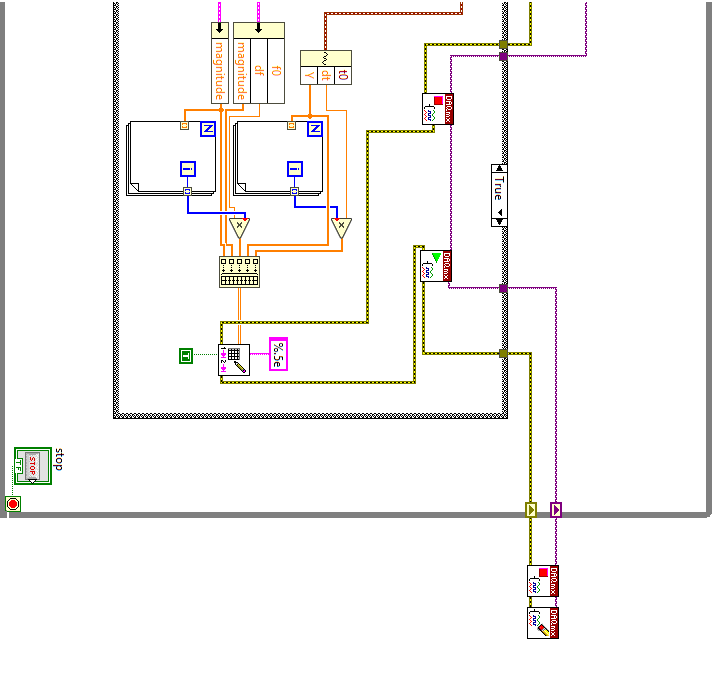
\includegraphics[width=\textwidth]{pic/messstruktur2.png}	
			\caption{Labview VI zur Messung, Spektralanalyse und Speicherung eines eingehenden Signals.}
			\label{fig:messstruktur}
		\end{figure}
		
		\thispagestyle{empty}
		Ähnlich zu dem DAQ-Assistant sind hier die Eingänge für Anzahl der Datenpunkte und Messrate vertreten.
		Die VIs, welche die Funktionen des DAQ-Assistants ersetzen sollen sind die DAQmx-VIs, welche in Reihe geschaltet werden.
		Als Eingang in das erste DAQmx-VI wir der Kanal übergeben von dem das Signal empfangen werden soll, welcher hier "physical channel" heißt.
		Bei dem verwendeten Computer handelte es sich bei diesem Kanal um "Dev3/ai0".
		Da Spannungen im differentiellen Modus gemessen werden sollten wurden "AI Voltage" und "Differential" als Modus bzw. konstanter Eingang an das DAQmx-VI gelegt. 
		Um die gemessene Spannungen variabel zu begrenzen wurden zusätzlich Controls angebracht.
		Die Benennung dieser mit "minimum value" und "maximum value" entstammt der voreingestellten Namen der Eingänge des DAQmx-VIs.
		In einer späteren Version wurden die englischen Namen durch deutsche ersetzt.
		Von den Ausgängen dieses VIs gehen nur der Signalkanal und ein Fehlerkanal durch, welche sich von hier aus bis ans Ende der Messstruktur durch alle DAQmx-VIs ziehen.
		
		Das zweite DAQmx-VI dient als Taktgeber für die Aufnahme des Signals, deswegen der Modus "Sample Clock".
		Ihm werden einerseits der Signalkanal und der Fehler übergeben, andererseits auch die Messrate "rate" und die doppelte Anzahl der Datenpunkte "samples per channel", damit der CPU weniger ausgelastet wird. 
		Mit dem letzten und konstanten Eingang "Continuous Samples" wird festgelegt, wie die Daten aufgenommen werden.
		Da der Funktionsgenerator kontinuierlich ein Signal ausgibt, soll auch so lange getaktet werden, bis der Nutzer das Programm beendet.
		
		Das nächste DAQmx-VI ist nur für den Start des Messvorgangs zuständig.
		Von dort aus geht es in eine while-Schleife mit Stopp-Knopf, damit das Programm jederzeit von dem Benutzer beendet werden kann, ohne dass ein Stopp von Labview erzwungen werden muss.
		In dieser while-Schleife ist das erste Element ein weiteres DAQmx-VI.
		Dieses ist für das Lesen des Signals mit den vorgegebenen Parametern des Taktgebers verantwortlich.
		Es gibt ein dynamisches Array der Messdaten aus, welches mit Hilfe eines Waveform-Graphen auf der Frontplatte dargestellt werden kann.  
		Des Weiteren wird die Ausgabe für eine Spektralanalyse über zwei verschiedene Express-VIs genutzt. 
		Dabei wird bei einem mit dem sogenannten Hann-Fenster gearbeitet und bei dem anderen ohne.
		Das Hann-Fenster dient zur Manipulation der Messdaten, um die vorkommenden nicht ganzzahligen Frequenzen schärfer im Frequenzbild darzustellen, um den Leakage-Effekt zu unterdrücken, auf den später noch genauer eingegangen wird.
		
		Neben den Daten verläuft auch das Fehlerkabel durch die Express-VIs. 
		Falls ein Fehler in dem Programm auftritt dann wird aufgrund des VIs mit der Sprechblase eine Fehlermeldung ausgegeben und der Nutzer wird gefragt, ob das Programm weiterlaufen oder gestoppt werden soll.
		
		Um die ermittelten Daten für das Zeitbild und das Frequenzbild zu speichern wird die Case-Struktur nach der Spektralanalyse eingebaut.
		Wird auf den Speicherknopf auf dem Frontpanel gedrückt, so wird der in Abb. \ref{fig:messstruktur} dargestellte Fall durchgeführt.
		Andernfalls der in Abb. \ref{fig:messstruktur_case} dargestellte Fall, in dem das Programm einfach weiterläuft.
		\begin{figure}[H]
			\centering
			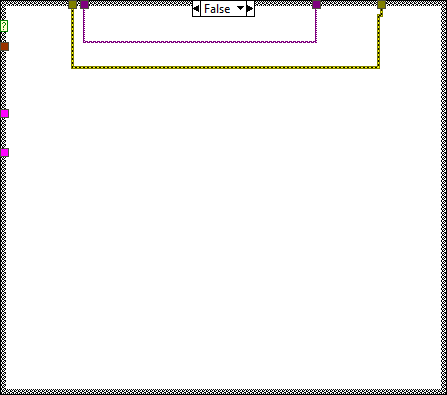
\includegraphics[width=0.5\textwidth]{pic/messstruktur_case.png}	
			\caption{Case der Messstruktur VI für den Fall, dass nicht gespeichert werden soll.}
			\label{fig:messstruktur_case}
		\end{figure}
	
		Im Falle des Speicherns hingegen wird das Lesen der Daten über ein DAQmx-VI angehalten, damit überhaupt ein fester Datensatz gespeichert werden kann.
		Um die Daten zu erhalten werden das Signal des Zeitbildes und der Frequenzbilder in Waveform-Builder gegeben um die einzelnen Parameter zu erhalten.
		Damit die Zeit $t_i$ und die Frequenz $f_i$ dargestellt werden können, werden die Differentiale d$t$ und d$s$ über for-Schleifen $i$ mal aufaddiert.
		Aus diesen Zeiten und Frequenzen werden mit ihren jeweiligen Amplituden (\si{\volt} im Zeitbild und \si{\decibel} im Frequenzbild, mit und ohne Hann-fenster) in ein Array gegeben und in ein VI gegeben, welches eine Datei ausgibt, in dem das Array mit $i$ Zeilen und den fünf Spalten für die einzelnen Parametern ausgegeben wird.
		An diesem VI lässt sich auch das Format der Daten darstellen, hier wurde "\%.5e" gewählt für eine Ausgabe wie in Tab. \ref{tab:speichern} für die exponentielle Schreibweise und fünf Nachkommastellen.	
		\begin{table}[ht]
			\centering
			\begin{tabular}{S S S S S}
				
				\text{0,00000E+0} &	\text{0,00000E+0} &	\text{1,21707E+0} &	\text{-4,15539E+1} &	\text{-5,78080E+1}\\
				\text{1,00000E-3} &	\text{1,00000E+0} &	\text{-6,34577E-1} &	\text{-3,99954E+1} &	\text{-6,09291E+1} \\
				\text{2,00000E-3} &	\text{2,00000E+0} &	\text{-2,24044E+0} &	\text{-4,00174E+1} &	\text{-9,43314E+1} \\
				\text{3,00000E-3} &	\text{3,00000E+0} &	\text{-2,98161E+0} &	\text{-4,00395E+1} &	\text{-8,78620E+1} \\
				$\colon$ \\		
				$\colon$ \\		
			\end{tabular}
			\caption{Beispielausgabe nach Nutzung der Speicherfunktion der Messstruktur.}
			\label{tab:speichern}
		\end{table}
		Eine automatische Benennung der Spalten ist hierbei nicht möglich, weswegen verfolgt werden muss welcher Wert an welcher Stelle in das Array eingefügt wird.
		
		Danach wird die Schleife wiederholt bis sie durch Betätigen des Stopp-Knopfes verlassen wird.
		Nach zwei weiteren DAQmx-VIs wird das Programm dann beendet.
		
	\subsection{Abtastung mit der Messstruktur}
	
		Mit der vorerst fertigen Messstruktur sollte nun abgetastet werden.
		Die Abbildungen \ref{fig:abtast_1kHz} bis \ref{fig:abtast_250,5Hz} stellen verschiedene Fälle dar.
		Der Verlauf in Abb. \ref{fig:abtast_1kHz} stellt den Fall der Unterabtastung dar.
		Hierbei entspricht die Frequenz der Messung mit der Signalfrequenz des Funktionsgenerator überein.
		Um das Abtasttheorem zu erfüllen, müsste jedoch mit mindestens der doppelten Frequenz abgetastet werden, weswegen hierbei keine Schwingung sondern nur ein annähernd linearer Verlauf im Zeitbild zu erkennen ist.
		Im Falle einer Messung mit exakt gleicher Frequenz wäre jedoch ein konstanter Verlauf zu erwarten, dies schließt auf einen Unterschied zwischen der Frequenz des Funktionsgenerators und der Messrate, obwohl beide auf den selben Wert eingestellt waren.
		
		Abb. \ref{fig:abtast_5Hz} verdeutlicht die Ungenauigkeit bei der Messung weiter.
		Hier war der Funktionsgenerator auf \SI{5}{\hertz} eingestellt, gemessen wurde jedoch ein breites Spektrum an Frequenzen, bei denen die am stärksten vorkommenden Frequenzen zwischen \SIrange{5}{6}{\hertz} liegen.
		
		Insbesondere die Darstellung im Frequenzbild von Signalen mit nicht ganzzahligen Frequenzen stellt bei vorliegender Messtechnik ein Problem dar.
		Vergleicht man die Abbildungen \ref{fig:abtast_250Hz} und \ref{fig:abtast_250,5Hz}, so ist bereits im Zeitbild zu erkennen, dass im nicht ganzzahligen Fall, bei einer Frequenz, die lediglich \SI{0,5}{\hertz} über der anderen liegt ein deutlich anderes Bild zu sehen ist, obwohl es sich bei beiden um einfache Sinusschwingungen mit jeweils nur eine Frequenz handeln sollte.
		Aufgrund der groß gewählten Frequenzen ist die Sinusform in Abb. \ref{fig:abtast_250Hz} kaum zu erkennen, jedoch lässt sich anhand der Amplituden ein Muster erkennen, welches einem einfachen Sinus deutlich mehr ähnelt als das in Abb. \ref{fig:abtast_250,5Hz}.
		
		Betrachtet man nun die Frequenzbilder, so fällt zunächst im Fall ohne Hann-Fenster auf, dass bei dem \SI{250}{\hertz}-Signal eine Frequenz noch recht deutlich heraus sticht.
		Bei dem \SI{250,5}{\hertz}-Signal weitet sich dieser Frequenzpeak jedoch auf und die Frequenz des Signals lässt sich somit deutlich schlechter erfassen.
		Dies nennt man Leakage-Effekt.
		Um dieses "Ausschmieren" zu verhindern, kann das Signal mit Hilfe einer sogenannten Fensterfunktion manipuliert werden.
		In den Abbildungen werden hier Hann-Fenster verwendet.
		Vergleicht man die Frequenzbilder mit Hann-Fenster in den Abbildungen \ref{fig:abtast_250Hz} und \ref{fig:abtast_250,5Hz} so fällt auf, dass der Leakage-Effekt deutlich geschwächt auftritt, dafür aber verstärktes Rauschen in den umliegenden Frequenzbereichen zu erkennen ist.
		Dieses Rauschen jedoch liegt weit unter dem gewünschten Frequenzpeak bei ca. \SI{-80}{\decibel} und ist demnach zu vernachlässigen.
		
		\begin{figure}[H]
			\centering
			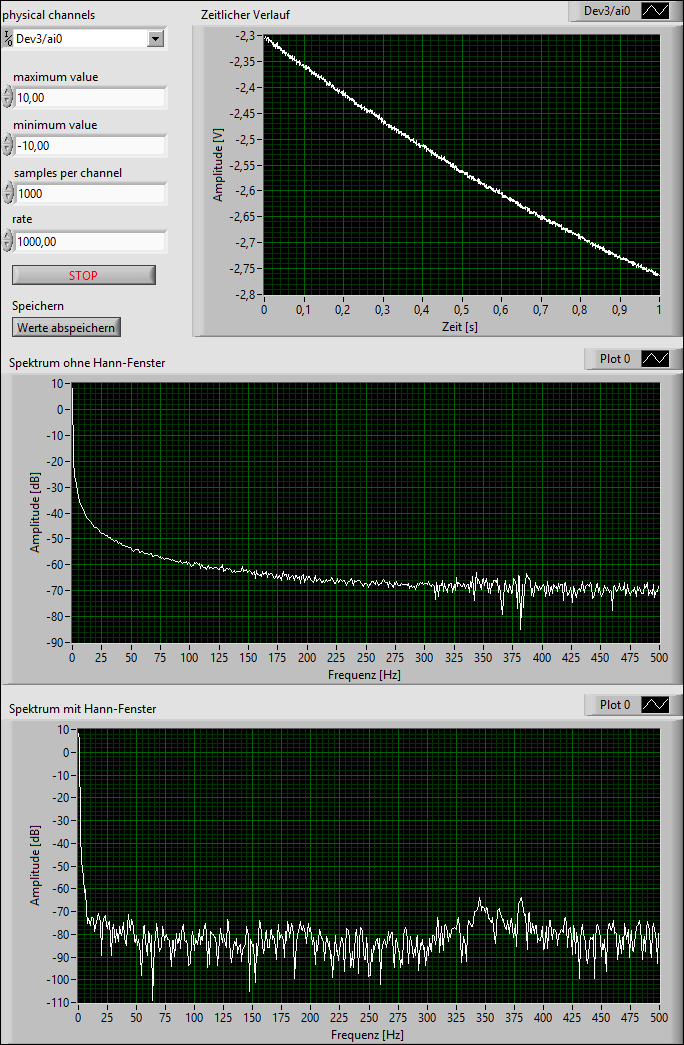
\includegraphics[width=0.85\textwidth]{pic/abtast_1kHz.png}	
			\caption{Frontpanel der Messstruktur bei eingehendem Sinussignal mit Frequenz \SI{1}{\kilo\hertz} und voreingestellten Parametern für Messrate etc.}
			\label{fig:abtast_1kHz}
		\end{figure}
		
		\begin{figure}[H]
			\centering
			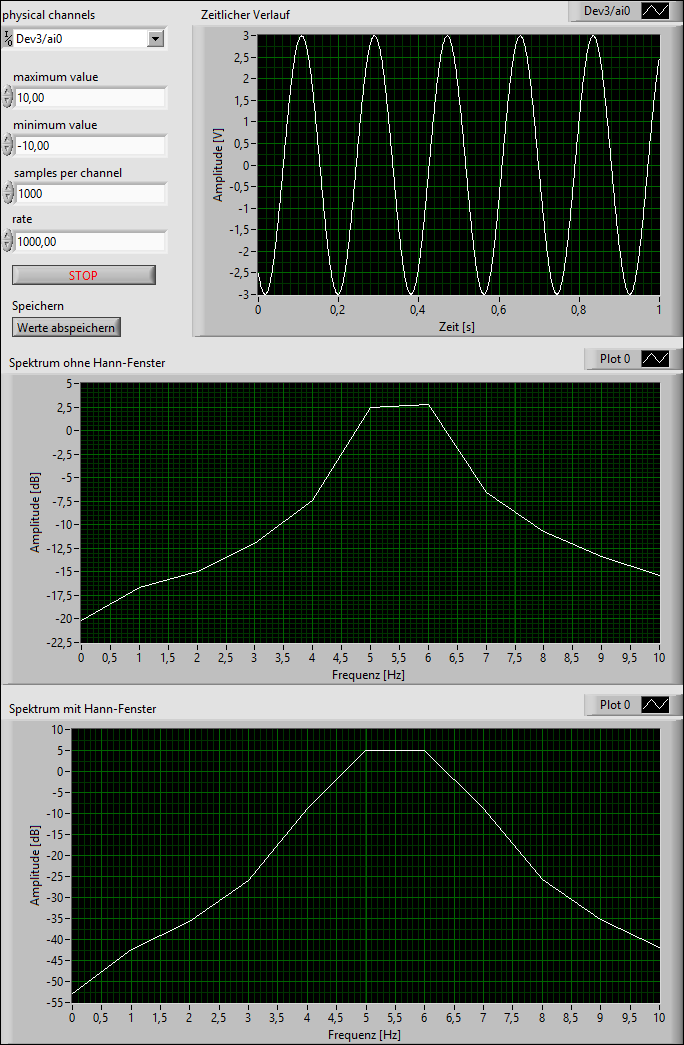
\includegraphics[width=0.85\textwidth]{pic/abtast_5Hz.png}	
			\caption{Frontpanel der Messstruktur bei eingehendem Sinussignal mit Frequenz \SI{5}{\hertz} und voreingestellten Parametern für Messrate etc.}
			\label{fig:abtast_5Hz}
		\end{figure}
			
		\begin{figure}[H]
			\centering
			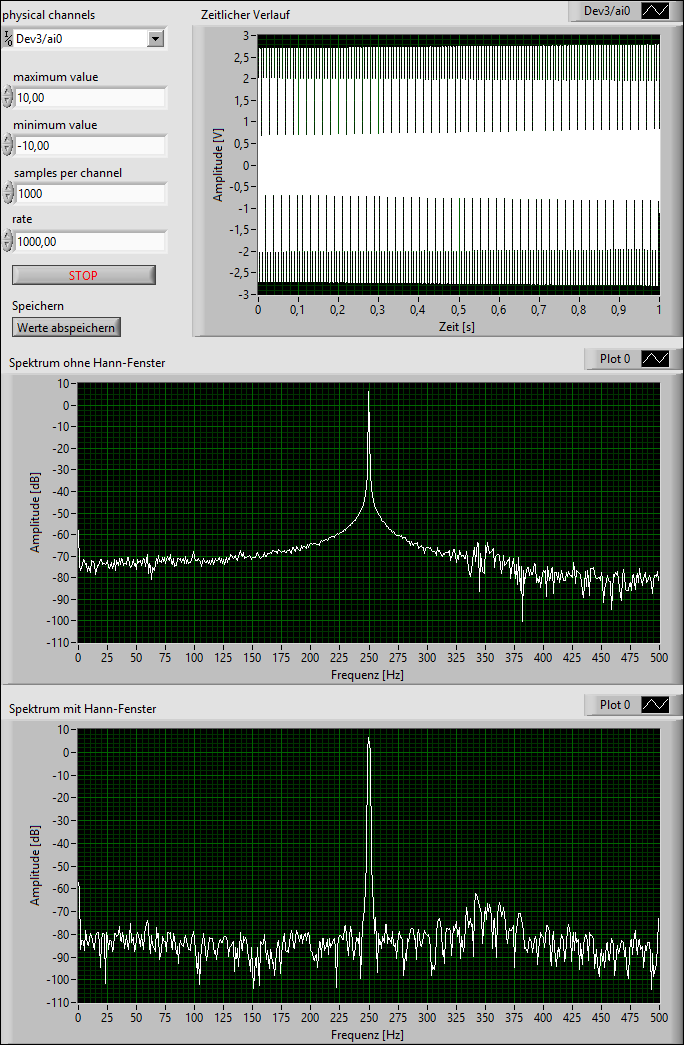
\includegraphics[width=0.85\textwidth]{pic/abtast_250Hz.png}	
			\caption{Frontpanel der Messstruktur bei eingehendem Sinussignal mit Frequenz \SI{250}{\hertz} und voreingestellten Parametern für Messrate etc.}
			\label{fig:abtast_250Hz}
		\end{figure}
	
		\begin{figure}[H]
			\centering
			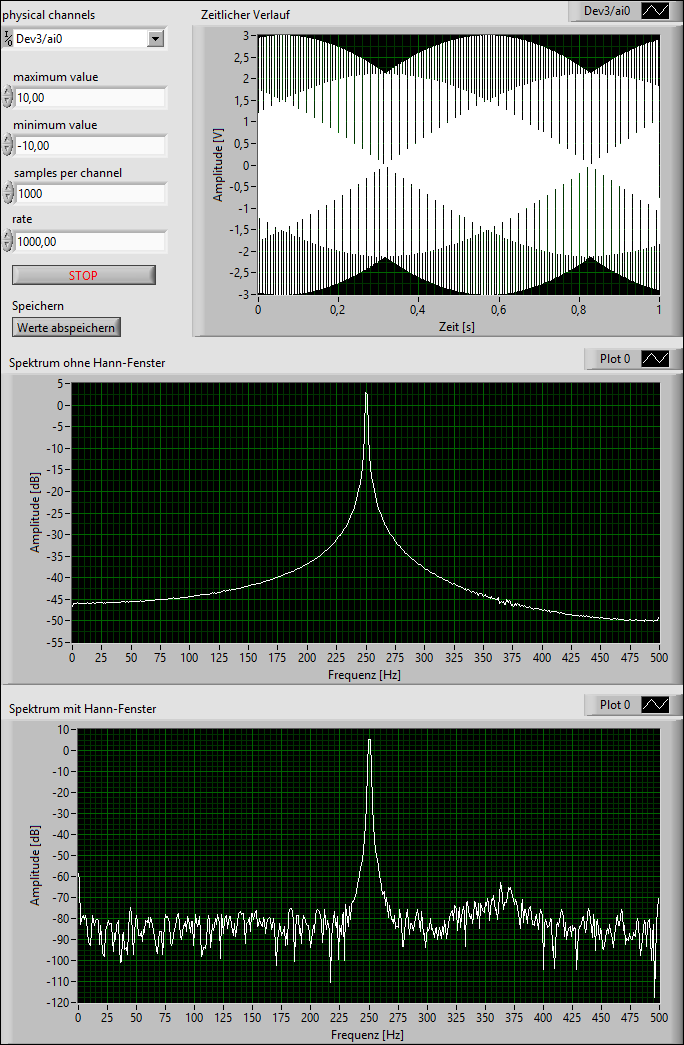
\includegraphics[width=0.85\textwidth]{pic/abtast_250,5Hz.png}	
			\caption{Frontpanel der Messstruktur bei eingehendem Sinussignal mit Frequenz \SI{250,5}{\hertz} und voreingestellten Parametern für Messrate etc.}
			\label{fig:abtast_250,5Hz}
		\end{figure}

\newpage
\section{Modulation}
	
	Als nächstes sollte der Funktionsgenerator durch die computereigene Soundkarte ersetzt werden.
	Um einen Schritt weiter zu gehen, sollte das Signal, welches der Soundkarte über ein Labview VI übergeben wird, amplitudenmoduliert sein.
	
	\subsection{Amplitudenmodulation}
	
		Das VI, welches ein amplitudenmoduliertes Signal erzeugt und von der Soundkarte ausgeben lässt ist in Abb. \ref{fig:am} dargestellt.
		Die VIs, welche für die Soundkartenausgabe zuständig sind, sind mit einem Lautsprechersymbol gekennzeichnet. 
		Wie auch bei der Messtruktur verläuft von dem ersten dieser VIs eine Fehlerleitung, damit eine Fehlermeldung ausgegeben werden kann, falls in dem Programm ein Fehler auftritt.
		Da auch hier ein kontinuierliches Signal gesendet werden soll, wird der Modus "Continuous Samples" für die Ausgabe festgelegt.
		Bei den drei Konstanten welche neben dem Modus in das Sound-VI gegeben werden handelt es sich um Frequenz, Anzahl der Kanäle und Bits.
		Mit den gewählten Werten von \SI{44100}{\hertz}, einem Kanal und 16 Bits wird der Ton im Mono-Format und mit CD-Qualität ausgegeben, welche die eingebaute Soundkarte unterstützt.
		Das Sound-VI nach der Übergabe der Parameter startet die Ausgabe und von dort wird die Schleife betreten, in der das Signal entsteht.
		Zu erkennen sind bereits Controls für das zu modulierende Signal, wie auch für den Träger.
		Hierzu liegt dem Aufbau folgende Formel zu Grunde:
		\begin{align}
			\label{eq:AM1} S_\text{AM}(t) &= (m \cdot S(t) + 1) \cdot T(t) \\
			\label{eq:AM2} \text{mit dem Signal} \quad S(t) &= A_1 \cdot \sin{(2\pi f_1 t)} + A_2 \cdot \sin{(2\pi f_2 t)}\\
			\label{eq:AM3} \text{und dem Träger} \quad T(t) &= s_\text{T} \cdot \sin{(2\pi f_\text{T} t)}.
		\end{align} 
		Aufgrund der Beschränkung der Soundkarte auf Signale mit maximaler Amplitude von einem Volt, wird der Modulationsgrad $m$ variabel gehalten, aber $s_\text{T}$ auf $\frac{1}{mA_1 + mA_2 + 1}$ normiert. 
		$A_{1/2}$ sind dabei die Amplituden der beiden Sinusschwingungen aus denen das zu modulierende Signal besteht und $f_{1/2}$ die jeweiligen Frequenzen, analog $f_\text{T}$ die Frequenz für den Träger.
		
		\newpage
		\thispagestyle{empty}
		\begin{figure}[H]
			\centering
			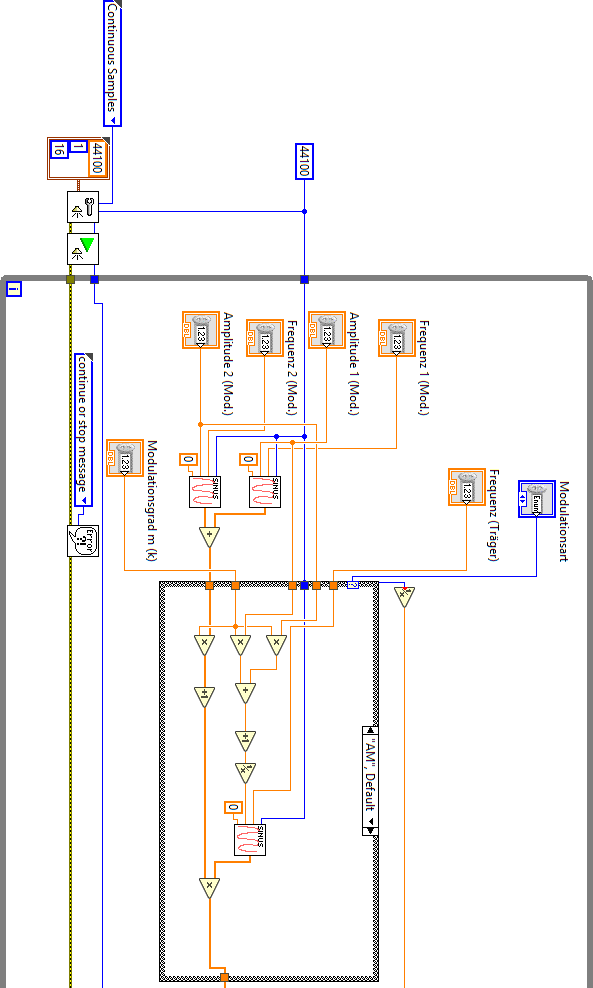
\includegraphics[width=0.95\textwidth]{pic/am1.png}
		\end{figure} 
		
		\begin{figure}[H]
			\centering
			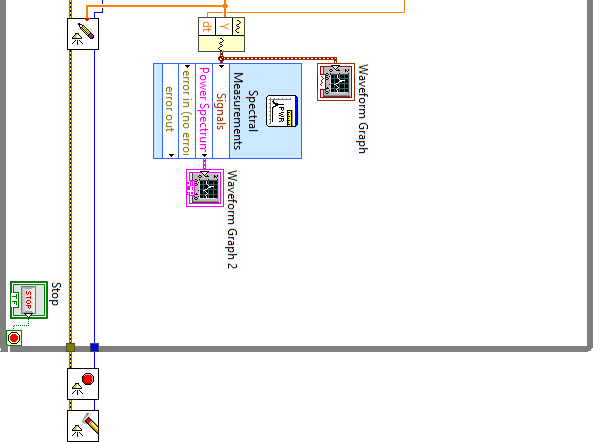
\includegraphics[width=0.95\textwidth]{pic/am2.png}
			\caption{Labview VI zur Erstellung eines amplitudenmodulierten Signals, welches von der Soundkarte ausgegeben und auf dem Frontpanel einstellbar und graphisch dargestellt wird.}
			\label{fig:am}	
		\end{figure} 
		
		\thispagestyle{empty}
		Das Signal $S(t)$ wird wie in Abb. \ref{fig:am} zu erkennen durch zwei der zuvor geschriebenen Sinus VIs verwirklicht.
		Zur besseren Aufnahme werden an dieser Stelle genau so viele Datenpunkte gewählt wie auch für die Sound VIs. 
		Analog zu der Frequenz hier 44100 Datenpunkte.
		Wie in der obigen Formel zu erkennen, werden die Phasen der Signale vernachlässigt und einfach gleich null gesetzt.
		Die eigentliche Modulation, also der Übergang von $S(t)$ zu $S_\text{AM}(t)$ findet in der Case-Struktur statt.
		Bei der Abbildung handelt es sich um das Endprodukt mit zudem eingebauter Frequenz- und Phasenmodulation zwischen denen hier unterschieden werden kann.
		Auf die anderen Cases wird später eingegangen, da diese erst im Nachhinein in das Modulations-VI hinzugefügt wurden.
		Zurück zu dem AM-Case: Hier sind die Rechnungen aus den Gleichungen \ref{eq:AM1} und \ref{eq:AM3} mit normierter Amplitude nachgestellt.
		Das Sinus-VI in dem Case stellt hierbei das Trägersignal dar, welches ebenfalls die Zahl der Datenpunkte von 44100 und Phase null besitzt.
		Zur Darstellung des modulierten Signals sind zudem ein Waveform-Builder und zwei damit verbundene Graphen hinzugefügt worden, damit man dieses im Zeit- und Frequenzbild auf dem Frontpanel betrachten kann.
		Natürlich verläuft das Signal nicht nur in den Waveform-Builder sondern auch in das Sound-VI, welches für die Ausgabe des eingehenden Signals über die Soundkarte führt.
		An dieser Stelle jedoch wurde der Ausgang zunächst falsch verkabelt, weswegen nicht das modulierte Signal ausgegeben wurde.
		Dieses Problem wurde erst am vierten und letzten Tag bei Erweiterung von Frequenz- und Phasenmodulation behoben.
		
		Wie auch bei der Messstruktur wird der Vorgang solange wiederholt bis der Stopp-Knopf auf dem Frontpanel gedrückt wird.  
		In Abbildung \ref{fig:am_example} ist dieses Frontpanel für ein Beispielsignal dargestellt.
		
		\begin{figure}[H]
			\centering
			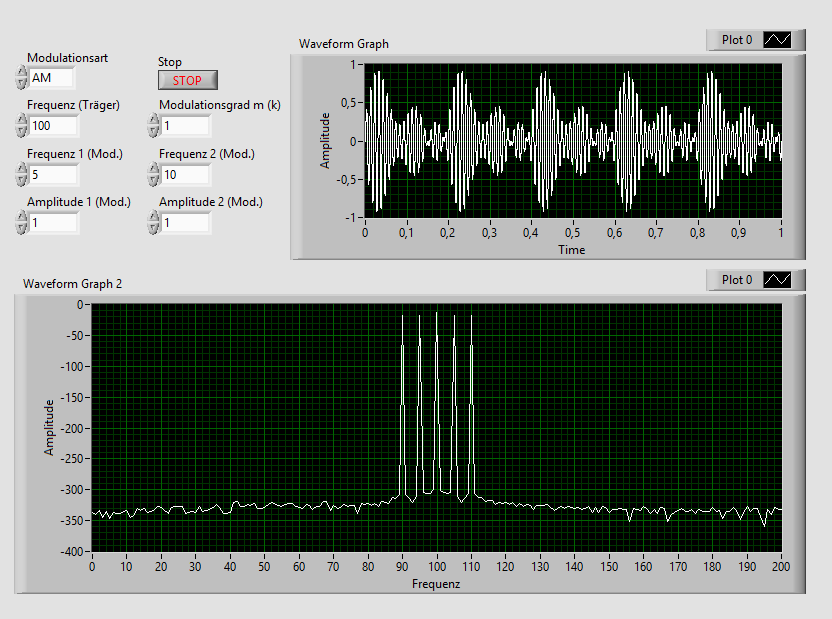
\includegraphics[width=0.95\textwidth]{pic/am_example.png}
			\caption{Frontpanel des Modulation-VIs bei AM mit Beispielsignal und einstellbaren Parametern.}
			\label{fig:am_example}	
		\end{figure} 
		
		Zu erkennen sind hier im Frequenzbild die Trägerfrequenz und die von der Amplitudenmodulation üblichen Seitenbänder links und rechts von der Trägerfrequenz pro Frequenz die im zu modulierenden Signal auftritt, sowie auch der schwebungsähnliche Verlauf im Zeitbild.
		Im Anhang (Abschnitt \ref*{sec:anhang}) sind weitere Beispiele verzeichnet.
		
	\subsection{Erweiterung der Messstruktur}
		
		Damit das nun modulierte Signal auch wieder demoduliert werden kann, musste die Messstruktur erweitert werden.
		Für die Amplitudenmodulation wurden hier drei verschiedene Arten der Demodulation integriert, von denen eine ausgewählt werden kann.
		Die Erweiterung von Abb. \ref{fig:messstruktur} ist in Abb. \ref{fig:messstruktur_dam} dargestellt.
		
		Bei den verschiedenen Demodulationsverfahren handelt es sich um die Quadratur, die Betragsbildung und die Multiplikation mit dem Träger, welche jedoch erst im Nachhinein am Morgen des vierten Tages hinzugefügt wurde.
		Um auch hier zu unterscheiden wurde eine Case-Struktur angelegt, bei der auch "keine Demodulation" eine Option ist.
		Der Fall der Quadratur ist bereits in Abb. \ref{fig:messstruktur_dam} dargestellt.
		Das Signal wird dabei einfach quadriert.
		Analog dazu wird bei der Betragsbildung einfach ein VI für den Betrag eingeschoben und bei keiner Demodulation die Kabel ohne weiteres durch den Case gezogen (vgl. Abb. \ref{fig:messstruktur_dam_case}). 
		Da nach den Rechenoperationen auch noch Frequenzen im Bereich doppelter Trägerfrequenz auftauchen, müssen diese gefiltert werden.
		Dies lässt sich leicht mit einem Tiefpass verwirklichen, solange das Verhältnis zwischen Trägerfrequenz und der des Ursprungssignals $f_\text{T} >> f_{1/2}$ gilt.
		
		Vor und nach dem Tiefpass wurden weitere Graphen für Zeit- und Frequenzbild eingefügt, um die einzelnen Schritte der Signalverarbeitung auch visuell auf dem Frontpanel darzustellen.
		Ansonsten ist das VI im wesentlichen das gleiche wie in Abb. \ref{fig:messstruktur}, nur die Speicherfunktion wurde noch um die zwei weiteren Datensätze nach Demodulation und nach Tiefpass erweitert.
		
		\newpage
		\pagestyle{empty}
		
		\begin{figure}[H]
			\centering
			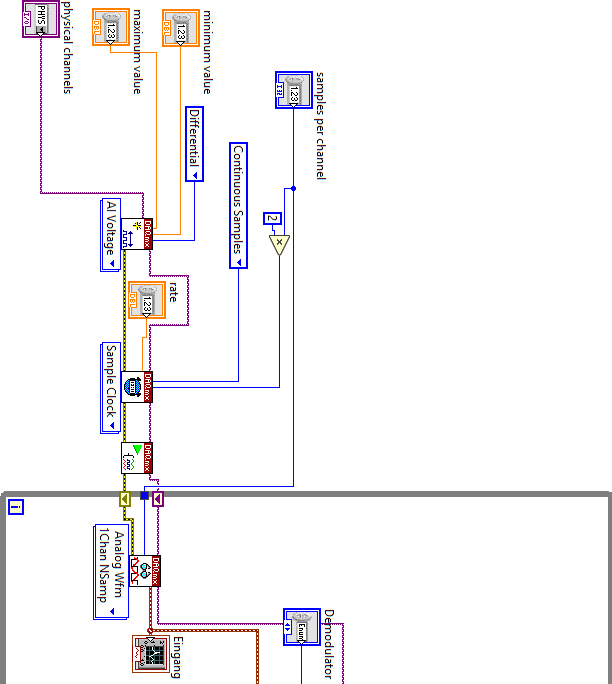
\includegraphics[width=\textwidth]{pic/messstruktur_dam1.png}
		\end{figure} 
	
			\begin{figure}[H]
			\centering
			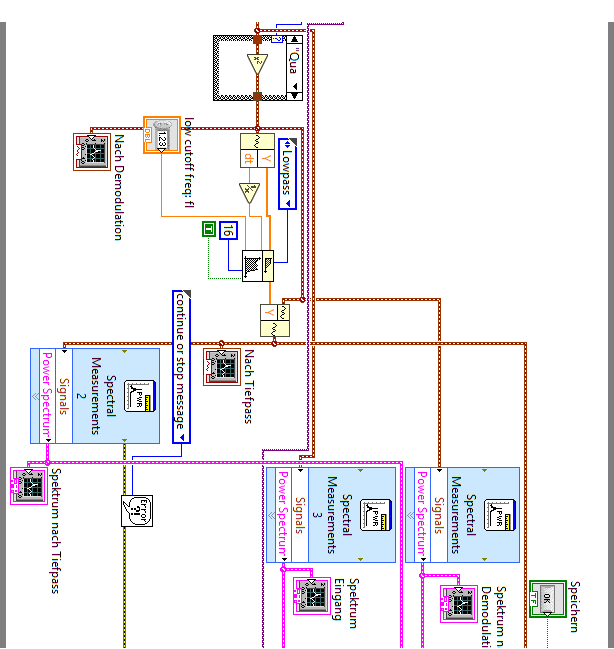
\includegraphics[width=\textwidth]{pic/messstruktur_dam2.png}
		\end{figure} 
	
		\begin{figure}[H]
			\centering
			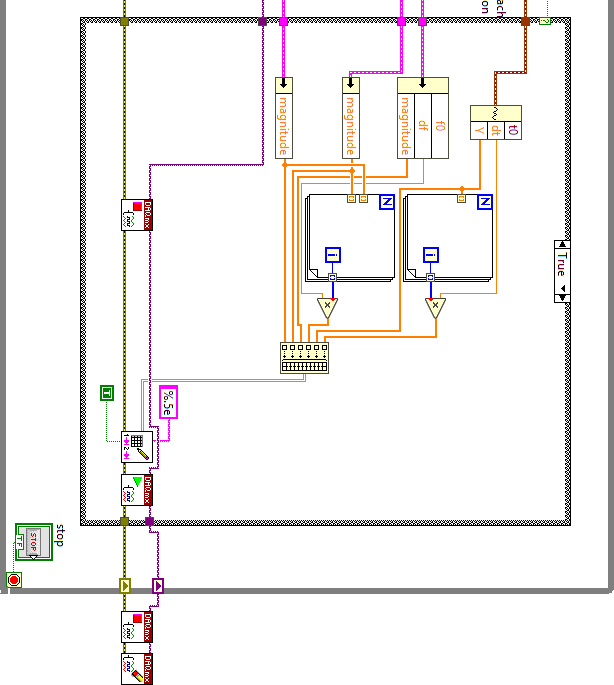
\includegraphics[width=\textwidth]{pic/messstruktur_dam3.png}
			\caption{Frontpanel des Modulation-VIs bei AM mit Beispielsignal und einstellbaren Parametern.}
			\label{fig:messstruktur_dam}	
		\end{figure} 
	
		\pagestyle{headings}
		
		\begin{figure}[H]
			\centering
			\begin{subfigure}[c]{0.45\textwidth}
				\centering
				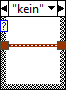
\includegraphics[width=0.3\textwidth]{pic/messstruktur_dam_case1.png}
				\subcaption{Case für den Fall ohne Demodulation.}
			\end{subfigure}
			\begin{subfigure}[c]{0.45\textwidth}
				\centering
				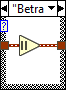
\includegraphics[width=0.3\textwidth]{pic/messstruktur_dam_case2.png}
				\subcaption{Case für den Fall von Demodulation über Betragsbildung.}
			\end{subfigure}	
			\caption{Alternative Fälle für den Case für die Demodulationsart in Abb. \ref{fig:messstruktur_dam}.}
			\label{fig:messstruktur_dam_case}	
		\end{figure}
	
		Wie bereits zuvor erwähnt war das Ende der Modulations-VI zunächst falsch verkabelt.
		Die Darstellungen für das Frontpanel der erweiterten Messstruktur wurden deshalb mit Hilfe eines von dem Funktionsgenerator ausgehenden Signals aufgenommen.
		Diese sind in den Abbildungen \ref{fig:dam_keine} bis \ref{fig:dam_betrag} jeweils einmal pro Demodulationsart aufgefasst.
		Für alle drei Abbildungen wurde das gleiche Signal von dem Funktionsgenerator verwendet mit Modulationsfrequenz $f_1= \SI{1}{\kilo\hertz}, f_2 = \SI{0}{\hertz}$, Trägerfrequenz $f_\text{T}\SI{1}{\kilo\hertz}$ und Modulationsgrad $m = 0,03$.
		Bei Abb. \ref{fig:dam_keine} entsprichen die Graphen nach der Demodulation selbstverständlich denen des Eingangssignals, da dieses nicht weiter verarbeitet wurde.
		Der Tiefpass erreicht an dieser Stelle nichts.
		Bei den Abbildungen \ref{fig:dam_quadrat} und \ref{fig:dam_betrag} hingegen kann man den Frequenzbildern nach der jeweiligen Demodulation entnehmen, dass nur die Frequenz des zu modulierenden Signals $f_1$, die Trägerfrequenz $f_\text{T}$ und das doppelte der Trägerfrequenz mit Seitenbändern vorliegt.
		An dieser Stelle erfüllt der Tiefpass seinen Zweck und in den Frequenzbildern ist die einzige Frequenz, die nicht in dem Rauschen bei $\leq \SI{-50}{\decibel}$ untergeht gerade die gesuchte Frequenzen des zu modulierenden Signals $f_1$.
		
		Weitere Beispiele sind auch für diese im Anhang (Abschnitt \ref{sec:anhang}) vorzufinden.
		
		\newpage
		\pagestyle{empty}
		\begin{figure}[H]
			\centering
			\begin{subfigure}[c]{\textwidth}
				\centering
				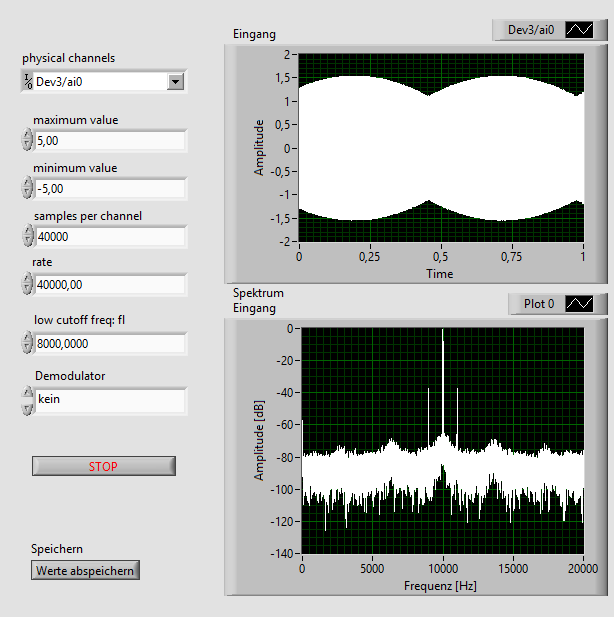
\includegraphics[width=0.7\textwidth]{pic/dam_keine1.png}
				\subcaption{Linke Seite des Frontpanels mit Parametern und Graphen für das Eingangssignal.}
			\end{subfigure}
			\begin{subfigure}[c]{\textwidth}
				\centering
				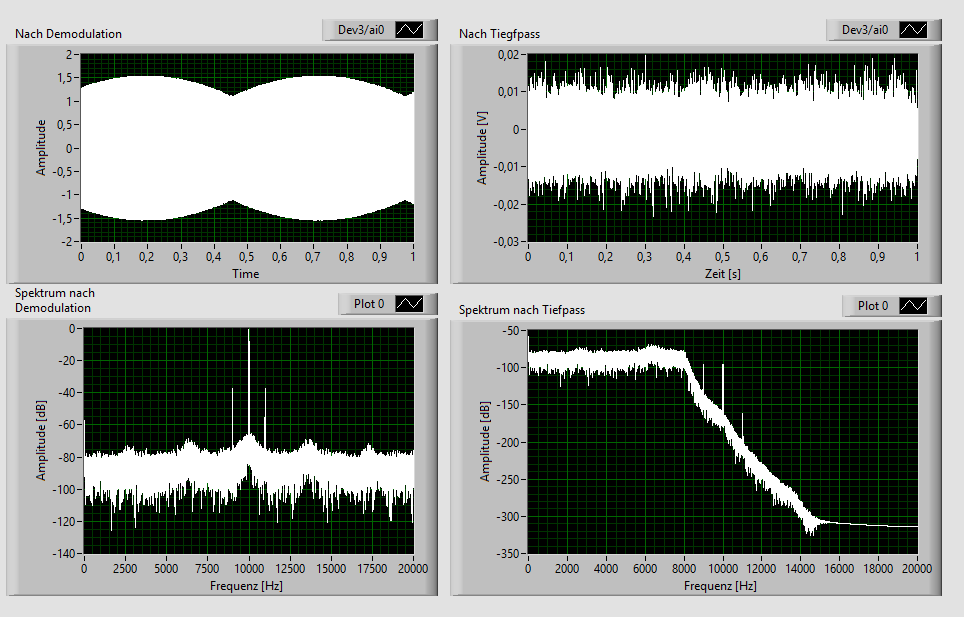
\includegraphics[width=0.9\textwidth]{pic/dam_keine2.png}
				\subcaption{Rechte Seite des Frontpanels mit Graphen für das demodulierte Signal vor und nach Tiefpass.}
			\end{subfigure}	
			\caption{Frontpanel der erweiterten Messstruktur bei eingehendem AM-Signal vom Funktionsgenerator mit Modulationsfrequenz $f_1= \SI{1}{\kilo\hertz}, f_2 = \SI{0}{\hertz}$, Trägerfrequenz $f_\text{T}\SI{1}{\kilo\hertz}$ und Modulationsgrad $m = 0,03$ ohne Demodulation.}
			\label{fig:dam_keine}	
		\end{figure} 
	
		\begin{figure}[H]
			\centering
			\begin{subfigure}[c]{\textwidth}
				\centering
				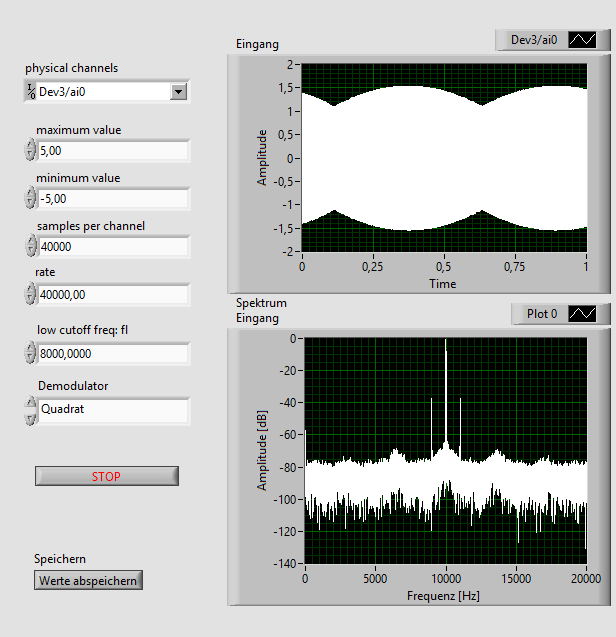
\includegraphics[width=0.7\textwidth]{pic/dam_quadrat1.png}
				\subcaption{Linke Seite des Frontpanels mit Parametern und Graphen für das Eingangssignal.}
			\end{subfigure}
			\begin{subfigure}[c]{\textwidth}
				\centering
				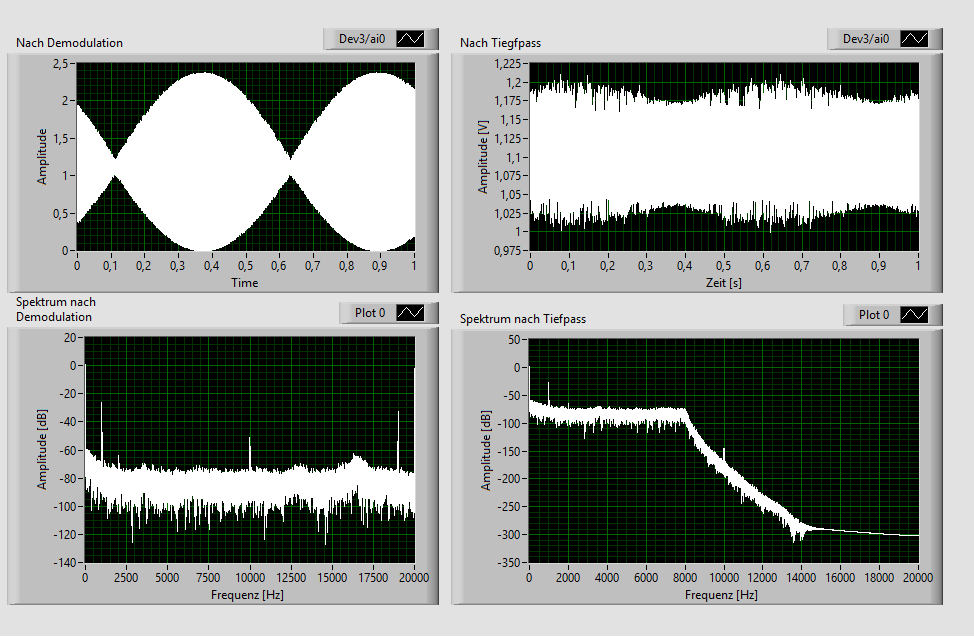
\includegraphics[width=0.9\textwidth]{pic/dam_quadrat2.png}
				\subcaption{Rechte Seite des Frontpanels mit Graphen für das demodulierte Signal vor und nach Tiefpass.}
			\end{subfigure}	
			\caption{Frontpanel der erweiterten Messstruktur bei eingehendem AM-Signal vom Funktionsgenerator mit Modulationsfrequenz $f_1= \SI{1}{\kilo\hertz}, f_2 = \SI{0}{\hertz}$, Trägerfrequenz $f_\text{T}\SI{1}{\kilo\hertz}$ und Modulationsgrad $m = 0,03$ ohne Demodulation.}
			\label{fig:dam_quadrat}	
		\end{figure} 
	
		\begin{figure}[H]
			\centering
			\begin{subfigure}[c]{\textwidth}
				\centering
				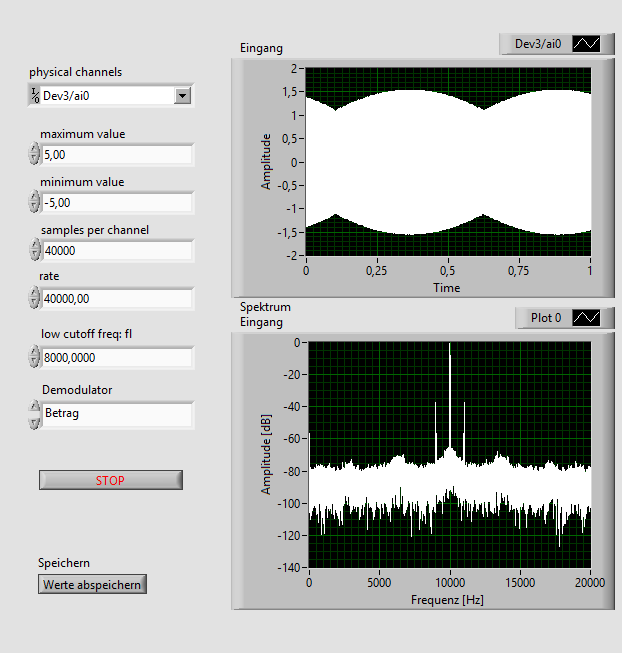
\includegraphics[width=0.7\textwidth]{pic/dam_betrag1.png}
				\subcaption{Linke Seite des Frontpanels mit Parametern und Graphen für das Eingangssignal.}
			\end{subfigure}
			\begin{subfigure}[c]{\textwidth}
				\centering
				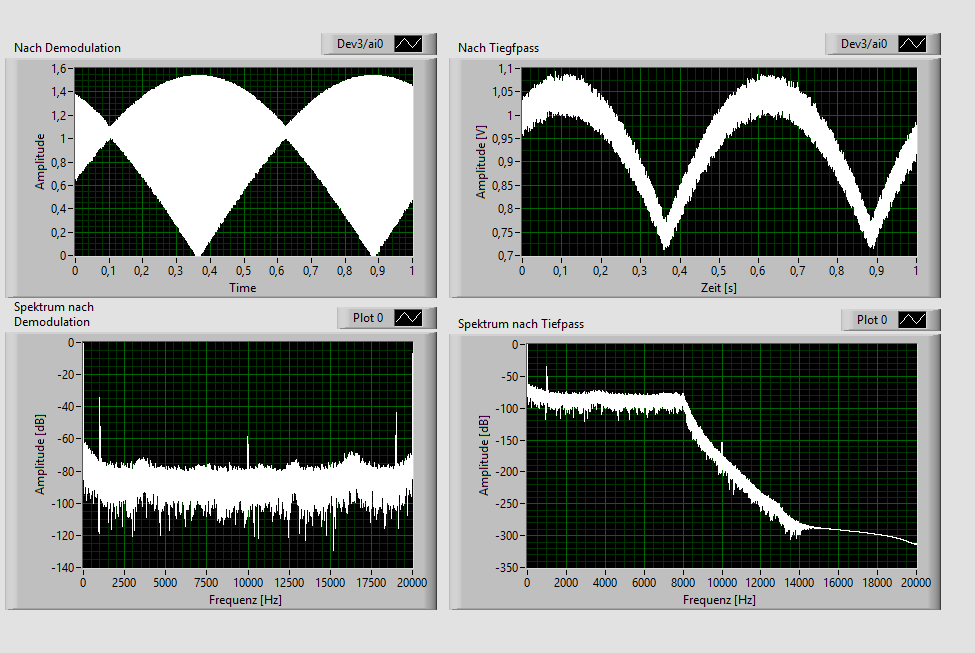
\includegraphics[width=0.9\textwidth]{pic/dam_betrag2.png}
				\subcaption{Rechte Seite des Frontpanels mit Graphen für das demodulierte Signal vor und nach Tiefpass.}
			\end{subfigure}	
			\caption{Frontpanel der erweiterten Messstruktur bei eingehendem AM-Signal vom Funktionsgenerator mit Modulationsfrequenz $f_1= \SI{1}{\kilo\hertz}, f_2 = \SI{0}{\hertz}$, Trägerfrequenz $f_\text{T}\SI{1}{\kilo\hertz}$ und Modulationsgrad $m = 0,03$ ohne Demodulation.}
			\label{fig:dam_betrag}	
		\end{figure} 